 \documentclass[a4paper,10pt]{article}
\usepackage[english]{babel}
\usepackage[utf8]{inputenc}
\usepackage[margin=1.5in]{geometry}
\usepackage{amsmath}
\usepackage{amsthm}
\usepackage{amsfonts}
\usepackage{amssymb}
\usepackage[usenames,dvipsnames]{xcolor}
\usepackage{graphicx}
\usepackage[siunitx]{circuitikz}
\usepackage{tikz}
\usepackage{hyperref}
\usepackage[numbers, square]{natbib}
\usepackage{fancybox}
\usepackage{epsfig}
\usepackage{soul}
\usepackage[framemethod=tikz]{mdframed}
\usepackage[shortlabels]{enumitem}
\usepackage[version=4]{mhchem}
\usepackage{fullpage}
\usepackage[nottoc, notlof, notlot]{tocbibind}
\setcounter{tocdepth}{2}

\def\hypothesis#1#2{{\color{purple}Hypothesis} {\color{blue}#1}: {\tt #2}}
\def\definition#1#2{{\color{purple}Definition} {\color{blue}#1} := {\tt #2}}
\def\ttt#1#2{{\tt{\color{black}#1} #2}}

%opening
\newtheorem{theorem}{Theorem}
\title{
\normalfont \normalsize 
\textsc{ENS Lyon} \\
[10pt] 
\rule{\linewidth}{0.5pt} \\[6pt] 
\huge Formalisation of the Delaunay Triangulation \\
\rule{\linewidth}{2pt}  \\[10pt]
}
\author{Clément Sartori}
\date{\normalsize 09/06/2017}

\begin{document}

\maketitle
\noindent
%Date Performed \dotfill December 31, 1999 \\
%Partners \dotfill Full Name \\
Advisor \dotfill Yves Bertot \\
%\title{Formalisation of the Delaunay triangulation}
%\author{Clément Sartori}


\maketitle

\begin{abstract}
  This report is the result of my internship at INRIA Sophia-Antipolis in the Marelle team, for the validation of the second year of my master's degree in Computer Science. During this internship I formalised Delaunay Triangulations in Coq. My code, although incomplete, can be found here : \href{https://github.com/Nemeras/StageDelaunay}{https://github.com/Nemeras/StageDelaunay}.
\end{abstract}

\tableofcontents{}

\newpage

\section{Introduction}
\rule{\linewidth}{0.5pt}

I did my second year of master's degree internship under the supervision of Yves Bertot at the INRIA Sophia-Antipolis in the Marelle team. The goal of this internship was to formalise Delaunay triangulations in the proof assistant {\sc{Coq}}.

The goal of this internship was to formalise the Delaunay triangulations in the {\sc{Coq}} proof assistant, that is, to try and find a minimal number of geometrical properties that had to be satisfied in order to get Delaunay triangulations. One of the goal of the internship was to stay as close as possible to Knuth's paradigm in \cite{Knuth92} with the CC system, by describing the biggest number of geometrical properties using only combinatorial properties such as the orientation predicate ``is left of''.

\subsection{Triangulations and Applications}

In geometry, a triangulation T of an object X of $\mathbb{R}^d$ is the partition of this object into simplices such that :
\begin{itemize}
\item the intersection of two simplices is either empty or a face of those simplices
\item every bounded set of $\mathbb{R}^{d}$ cuts a finite number of simplices of T
  \item the union of the simplices of T is X itself.
\end{itemize}

In the plane (where we stayed during this internship), the triangulation of a set of points is the partition of this set of points into triangles.\\

\begin{figure}
  \centering
  
  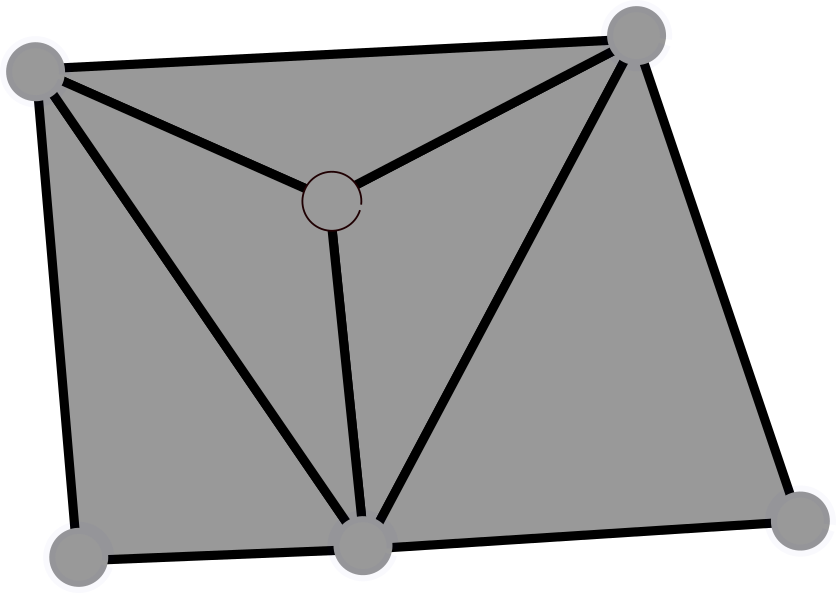
\includegraphics[scale=2]{Trig1}
  \caption{\label{Trig1} This is a triangulation}
\end{figure}

\begin{figure}
  \centering
  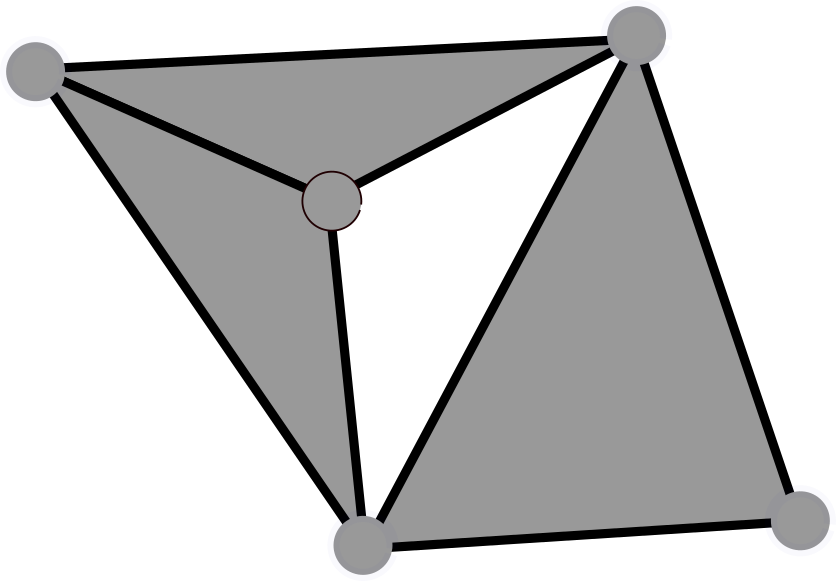
\includegraphics[scale=2]{NotTrig1}
  \caption{\label{NotTrig1} This is not a triangulation}
\end{figure}

\begin{figure}
  \centering
  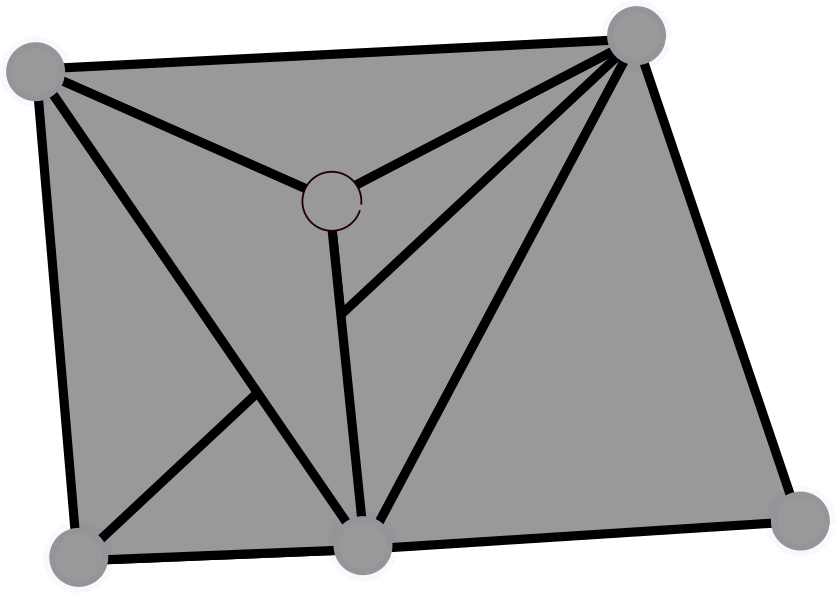
\includegraphics[scale=2]{NotTrig2}
  \caption{\label{NotTrig2} This is not a triangulation}
\end{figure}


More particularly, during this internship, we were interested in Delaunay triangulations : in the plane, a triangulation T of a set P of points is said to be a Delaunay triangulation if no point of P is in the circumcircle of a triangle of T.

Figure \ref{notDelaunay} for instance, is not a Delaunay triangulation.

\begin{figure}[h]
\centering
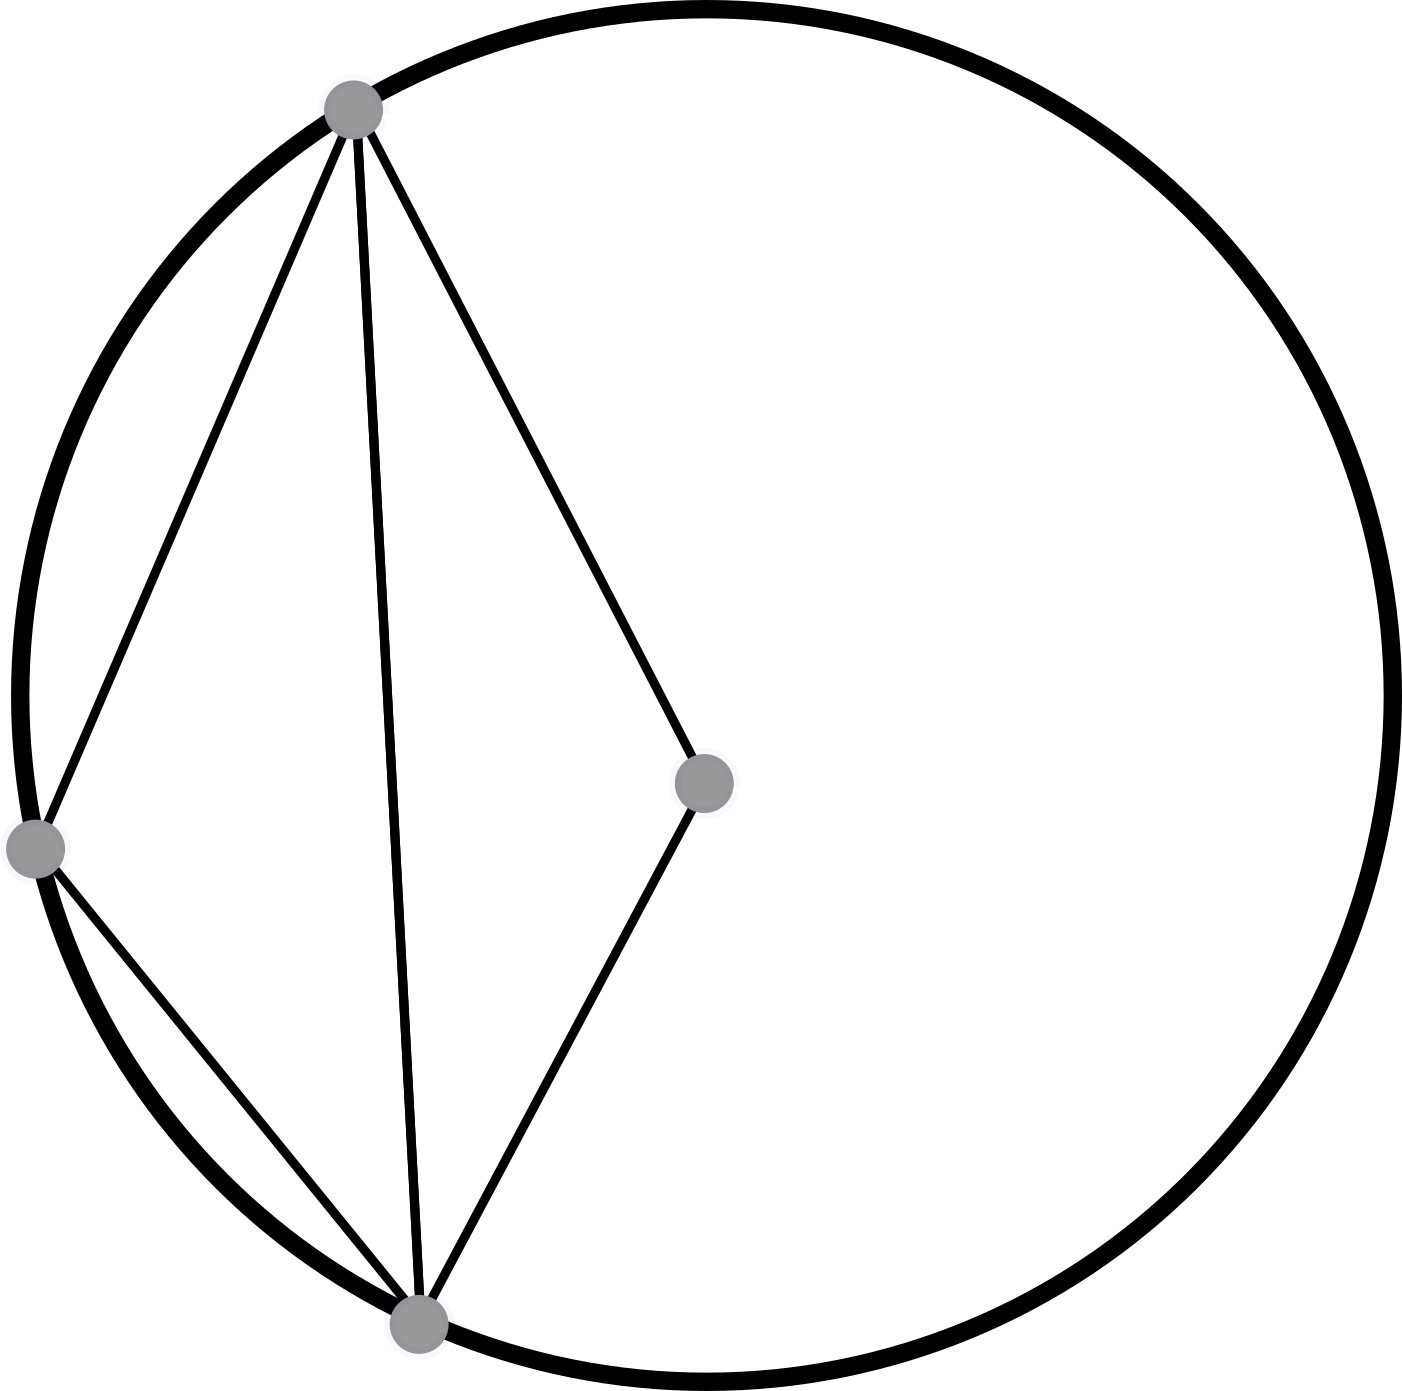
\includegraphics[scale=1]{dessin2}
\caption{\label{notDelaunay} Instance of a triangulation that is not a Delaunay triangulation}

\end{figure}

An example of domain where Delaunay triangulations are very useful is Robotics. Indeed, one of the interesting byproducts of Delaunay triangulations is the Voronoi diagram (the dual graph of the Delaunay triangulation) that can be very useful, for instance, to modelise cellular coverage maps \cite{CelCov}, or for path planning \cite{PathPla}.

\subsection{Coq/The Mathematical Component library}

Machine-checked proofs are a research domain which has more than forty years (see \cite{Automath}). As such, the domain acquired a certain maturity; however, the main problem stays the difficulty of use of proof assistants.

I wrote my formalisation of the Delaunay triangulation in the proof assistant {\tt Coq}, an environment and a language in which you can express and prove mathematical assertions and which automatically checks them. The advantage of {\tt Coq} (and proof assistants in general) is that, as long as you trust {\tt Coq}'s kernel, you can trust any {\tt Coq} proof. The choice of {\tt Coq} was very simple : {\tt Coq} is the most accomplished proof assistant in my opinion, and has the enormous advantage of having access to the {\tt Mathematical Component} library.

To make proofs simpler, I used the {\sc{Mathematical Component}} library and the extension of {\sc{Coq}}'s tactic language, {\sc{SSReflect}}. The goal of the {\sc{Mathematical Component}} library project is to create a library of mathematical results, so that those result are easily reusable in {\sc{Coq}}. Examples of successful application of the {\sc{Mathematical Component}} library and {\sc{SSReflect}} are the proof of the four-color theorem \cite{Gonthier08} and of the odd order theorem \cite{odd}.

\section{The Algorithm}
\label{algo}
\rule{\linewidth}{0.5pt}

The context of the algorithm studied is, given a set of points in a plane, how to compute the Delaunay triangulation of this set of points. The algorithm studied is an incremental algorithm in two parts : given an existing triangulation and a point, the algorithm consists in
\begin{enumerate}
\item Adding the point to the existing triangulation
\item Flipping the illegal edges to obtain a Delaunay triangulation.
\end{enumerate}

\subsection{Adding points}

In itself, adding the point to the existing triangulation is not a trivial problem, depending on whether the new point is in the convex hull of the existing points or not. In the litterature (\cite{Del}), for incremental algorithm, it is generally considered that the sites studied are inclosed within large triangles, which basically means that every new point will be in the convex hull of the previous ones. This was considered to be the case here. If this is not the case, then there is the need of an incremental algorithm to create convex hulls. The formalisation of such an algorithm has been done by David Pichardie in \cite{Hull}.

Thus, adding a new point P to a triangulation T, when the new point is in the convex hull of the triangulation, is a two step process :
\begin{enumerate}
\item The first step is to find the triangle t of the triangulation in which P is 
\item The second step is to replace t by three new triangles.
\end{enumerate}
\begin{figure}[h]
\centering
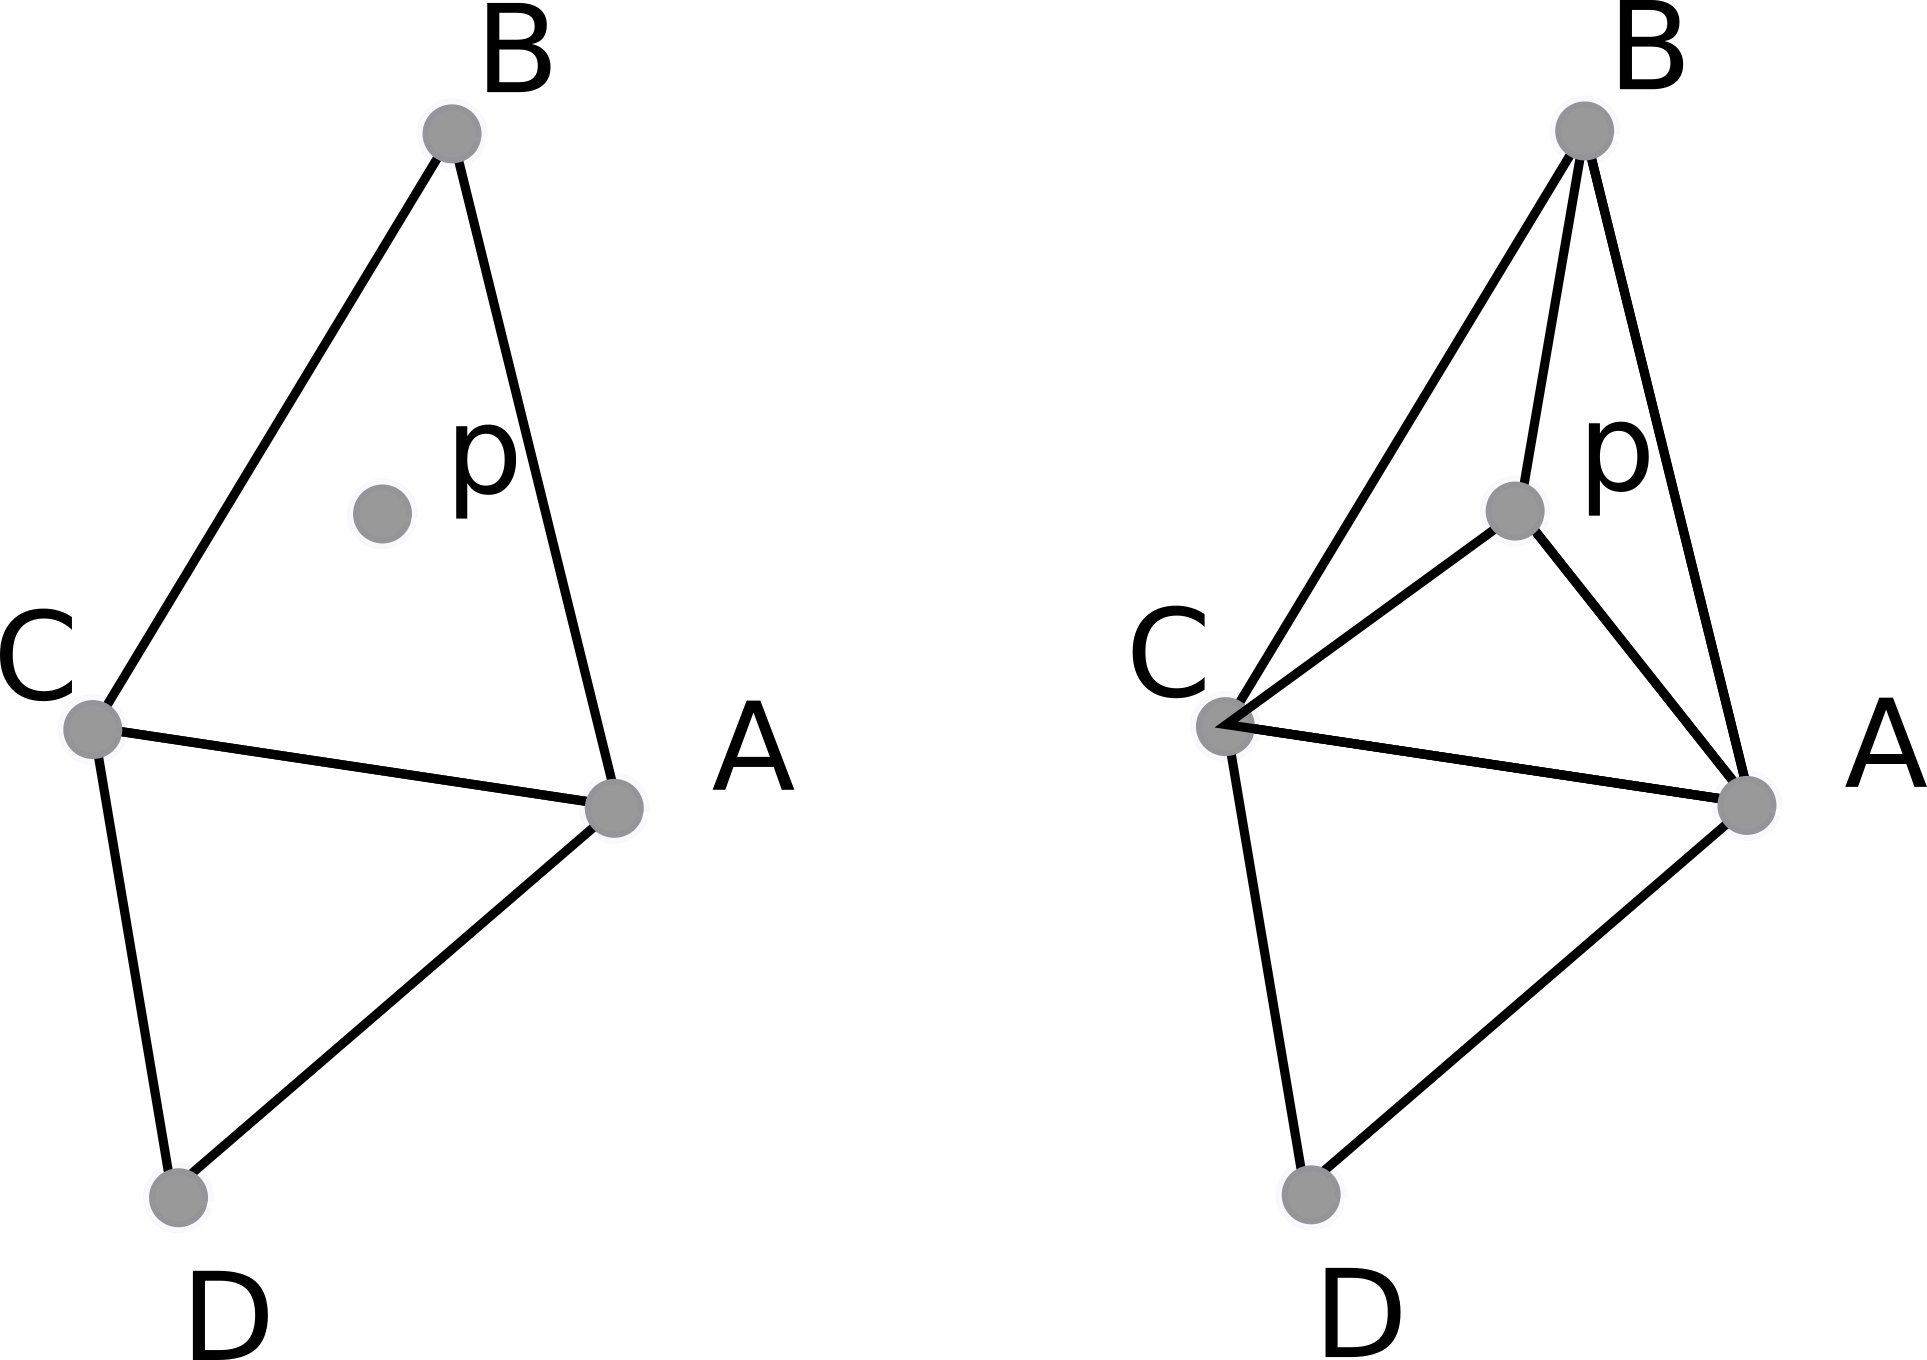
\includegraphics[scale=1]{adding}
\caption{Adding a point to a triangulation}
\end{figure}
\subsection{Flipping edges}

It is possible , from any triangulation of a set of point, to obtain a Delaunay triangulation by repeating the same step : for each pair of triangles that do not meet the Delaunay condition, flip the common edge of the triangles.

For instance, while Figure \ref{notDelaunay} was not a Delaunay triangulation, the result of an edge-flipping step, Figure \ref{DelaunayTriangulation}, however, is a Delaunay triangulation
\begin{figure}[h]
\centering

\includegraphics[scale=1]{dessin1}
\caption{\label{DelaunayTriangulation} Result of an edge-flipping step : example of Delaunay triangulation}
\end{figure}\\
This makes it possible to create a ``flipping'' algorithm : for any set of points, it is possible to obtain the Delaunay triangulation of this set of point by creating a random triangulation then applying this flipping step as many times as necessary.
\section{Formalisation of the Delaunay triangulation}
\rule{\linewidth}{0.5pt}

The goal of the formalisation is to stay as much as possible at a level where geometrical properties, predicates, etc, speak about mathematical concepts (for instance, points) as concepts (for instance, a point being a point versus a point being a pair of coordinates). Basically, the formalisation describes what properties every implementation of the concept should satisfy.

Here we describe a formalisation of the Delaunay triangulation. Any implementation should contain a type P for the points, a type T for the triangles, a type E for the edges, a type $\mathbb{R}$ for the coordinates of the points (a real integral domain where all elements are positive or negative).
Then , any implementation should contain basic functions :
\begin{itemize}
\item A function \ttt{vertices\_to\_edge}{} to create an edge from two points
\item A function \ttt{vertices\_to\_triangles}{} to create a triangle from three points
\item A function \ttt{vertex}{}  that returns the first, second or third vertex of a triangle
\item A function \ttt{xCoord}{} that returns the X coordinate of a point
\item A function \ttt{yCoord}{} that returns the Y coordinate of a point
\end{itemize}

Here, a choice has been made so that proofs are simpler : the order of the vertices of a triangle is important. This means that the triangle $abc$ won't be the same triangle than the triangle $bca$.

\subsection{Geometrical predicates}

Then, any implementation should also contain some geometrical predicates :
\begin{enumerate}
\item \ttt{is\_left\_of}{} and \ttt{is\_left\_or\_on\_line}{$a$ $b$ $c$} which test if the point $c$ is (strictly) left of the points $a$,$b$ e.g. if $a$,$b$,$c$ form a (strictly) well-oriented (counter-clockwise) triangle.
\item \ttt{in\_circle}{$p$ $a$ $b$ $c$} which tests if a point $p$ is in the circumcircle of the triangle described by $a$,$b$,$c$.
\item \ttt{in\_triangle}{$t$ $p$} and \ttt{in\_triangle\_w\_edges}{$t$ $p$} which test if $p$ is (strictly) in $t$.
  \item \ttt{is\_on\_line}{} which tests is 3 points are aligned.

\end{enumerate}

Those predicates easily come from another predicate : \ttt{oriented\_surface}{$a$ $b$ $c$}  which computes the oriented surface described by the three points $a$,$b$,$c$ :
\begin{itemize}
\item \ttt{is\_left\_of}{a b c = oriented\_surface a b c > 0}
  \item \ttt{is\_left\_or\_on\_line}{a b c = oriented\_surface a b c $\geq$ 0}
  \item \ttt{is\_on\_line}{a b c = oriented\_surface a b c = 0}
\item \begin{tabular}{ll}
       \ttt {in\_triangle}{t p = }& \ttt{}{is\_left\_of (vertex1 t) (vertex2 t) p} $\wedge$\\
        &\ttt{}{is\_left\_of p (vertex2 t) (vertex3 t)} $\wedge$\\
  & \ttt{}{is\_left\_of (vertex1 t) p (vertex3 t)}
      \end{tabular}
\item \begin{tabular}{ll}
       \ttt{in\_triangle\_w\_edges t p}{= }& \ttt{}{is\_left\_or\_on\_line (vertex1 t) (vertex2 t) p} $\wedge$\\
        & \ttt{}{is\_left\_or\_on\_line p  (vertex2 t) (vertex3 t)} $\wedge$\\
  & \ttt{}{is\_left\_or\_on\_line (vertex1 t) p (vertex3 t)}
      \end{tabular}
 \item \ttt{oriented\_triangle}{t = oriented\_surface (vertex1 t) (vertex2 t) (vertex3 t) $\geq$ 0} 
  \end{itemize}.

  The \ttt{is\_left\_of}{} predicate is inspired by Knuth's idea of CC systems \cite{Knuth92}.
  However, unlike him, we don't considere that our points are necessarily in general position. Thus, the opposite of \ttt{is\_left\_of}{a b c} is not \ttt{is\_left\_of}{b a c} but \ttt{is\_left\_or\_on\_line}{b a c}. A broader explanation of what happens to Knuth's axioms when degenerate cases (aligned points) can happen can be found in \cite{Hull}.

  \subsection{Hypotheses}
\label{Hypothesis}
We put assumptions (that have to be proven true for any implementation) on the implementations of the predicates/functions. Some are easy :
\begin{itemize}
\item \hypothesis{oriented\_surface\_xx}{$\forall$ x y, {\tt oriented\_surface x x y} = 0}.
\item \hypothesis{oriented\_surface\_circular}{$\forall$ a b c, oriented\_surface a b c = oriented\_surface c a b}.
\item \hypothesis{oriented\_surface\_change}{$\forall$ a b c, oriented\_surface a b c = - oriented\_surface b a c}.
\item \hypothesis{vertices\_to\_edge\_sym}{$\forall$ a b, vertices\_to\_edge a b = vertices\_to\_edge b a}.
  \item 
\hypothesis{vertices\_to\_triangle\_oriented}{$\forall$ a b c, oriented\_triangle (vertices\_to\_triangle a b c).}
\item\hypothesis{is\_on\_line\_trans}{$\forall$ a b c d, a != b $\rightarrow$ is\_on\_line a b c $\rightarrow$ is\_on\_line a b d $\rightarrow$
  is\_on\_line a c d}.
\item \hypothesis{vertices\_to\_triangle\_correct2}{\\$\forall$ p1 p2 p3, $\forall$ t,
          (t = vertices\_to\_triangle p1 p2 p3) ->
  ((p1 $\in$ vertex\_set t) $\wedge$ (p2 $\in$ vertex\_set t) $\wedge$ (p3 $\in$ vertex\_set t))}.

\end{itemize}
There are also assumptions on the functions that are made to link functions between each other : for instance, to explain what is the edge set of a strictly well-oriented triangle created thanks to vertices-to-triangle :

\hypothesis{edges\_set\_vertices\_to\_triangle:}
  {\\$\forall$ a b c, is\_left\_of a b c $\rightarrow$
    edges\_set (vertices\_to\_triangle a b c) =\\ 
                       $[$ fset (vertices\_to\_edge a b);
                           (vertices\_to\_edge a c);
                           (vertices\_to\_edge b c) $]$}.


Some assumptions are harder, because they are generalizations of Knuth's axioms or just come from harder geometrical facts. For instance:
\begin{itemize}
\item \hypothesis{is\_left\_of\_trans}{\\  \begin{tabular}{lll}
                                          $\forall$ a b c d q, &is\_left\_of a b c $\rightarrow$\\
                                           &is\_left\_of a b d $\rightarrow$\\
                                           &is\_left\_of a b q $\rightarrow$\\
                                           &is\_left\_of q b d $\rightarrow$\\
                                           &is\_left\_of d b c $\rightarrow$\\
                                           &is\_left\_of q b c 
           \end{tabular} }.
\\
\begin{figure}[h]
\centering
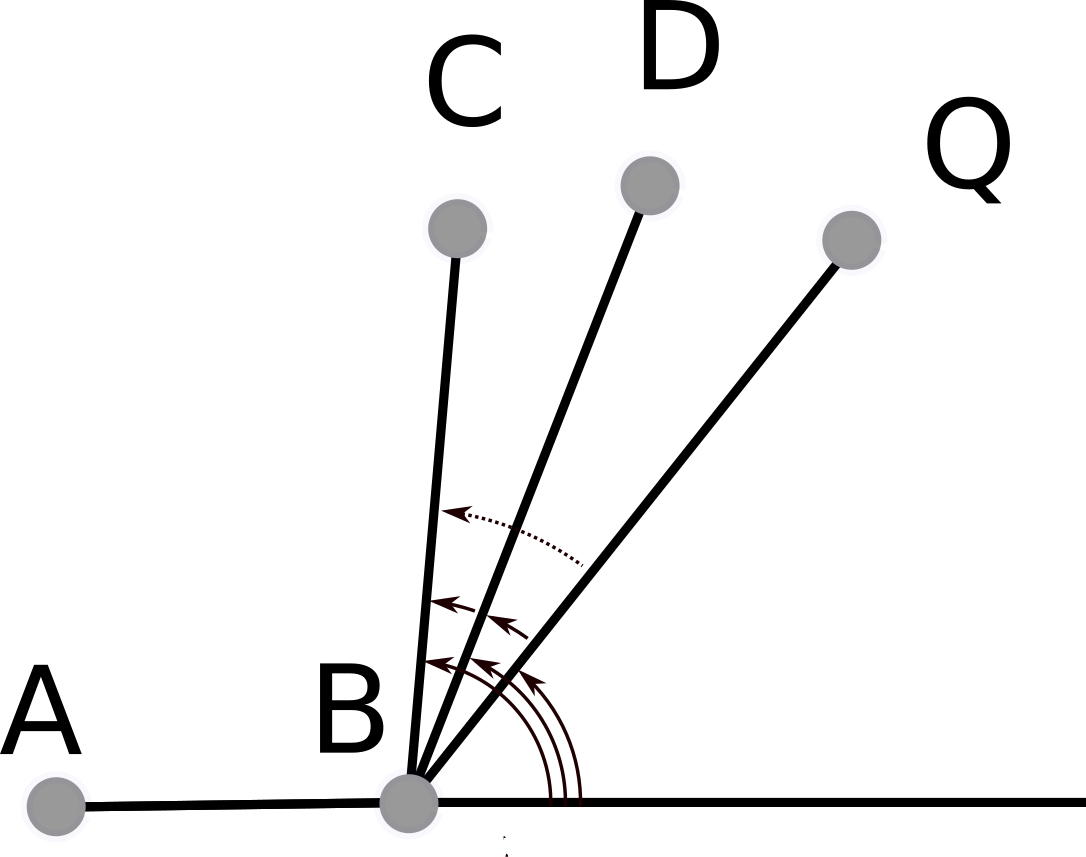
\includegraphics[scale=2]{Axiom5}
\caption{Knuth's 5$^{th}$ Axiom}
\end{figure}\\
The idea to understand this hypothesis is that we're sorting {\tt c d} and {\tt q} in a semi-plane defined by {\tt a} and {\tt b}.
\item \hypothesis{Axiom 4}{\\ \begin{tabular}{ll}
             $\forall$ a b c d,                  &is\_left\_of a b d $\rightarrow$\\
                                           &is\_left\_of b c d $\rightarrow$\\
                                           &is\_left\_of c a d $\rightarrow$\\
                                           &is\_left\_of a b c $\rightarrow$
           \end{tabular}}.
\begin{figure}[h]
\centering
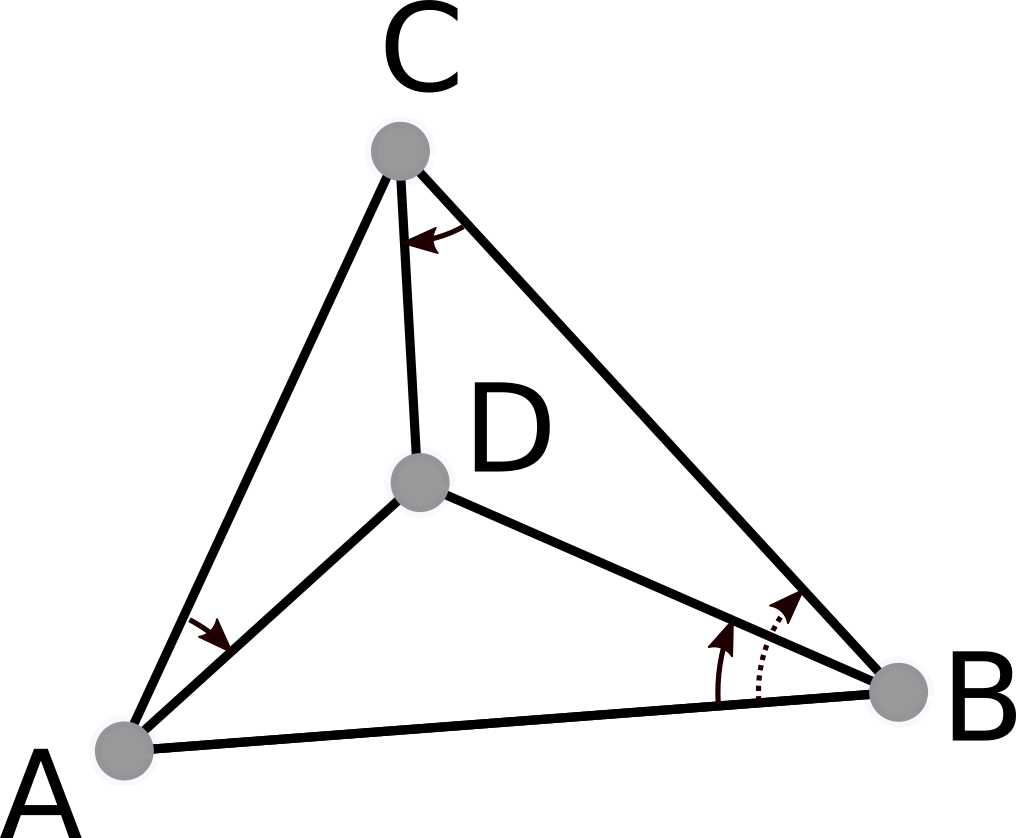
\includegraphics[scale=2]{Axiom4}
\caption{Knuth's 4$^{th}$ Axiom}
\end{figure}\\
\item \hypothesis{on\_line\_on\_edge}{(Figure \ref{edge_line}) :\\
  $\forall$ a b c, is\_left\_of a b c $\rightarrow$ $\forall$ q, is\_on\_line a c q $\rightarrow$ 
                                   is\_left\_of a b q $\rightarrow$\\ is\_left\_of b c q $\rightarrow$
                                   on\_edge (vertices\_to\_edge a c) q.}
\\
\begin{figure}[h]
\centering

\includegraphics[scale=2]{oloe}
\caption{\label{edge_line} Link between the geometrical predicates and being on an edge}
\end{figure}
\item \hypothesis{on\_edge\_on\_line}{(Figure \ref{edge_line}):\\
  $\forall$ a b c, is\_left\_of a b c $\rightarrow$
  $\forall$ q, on\_edge (vertices\_to\_edge a c) q $\rightarrow$ \\
           is\_on\_line a c q $\wedge$ is\_left\_of a b q $\wedge$ is\_left\_of b c q.}

       \item \hypothesis{intersection\_of\_lines}{(Figure \ref{intersection_line}) :
            $\forall$ a b c d,
is\_left\_of a b c -> is\_on\_line a b d ->
is\_on\_line a c d -> d = a.}
\\\begin{figure}[h]
\centering
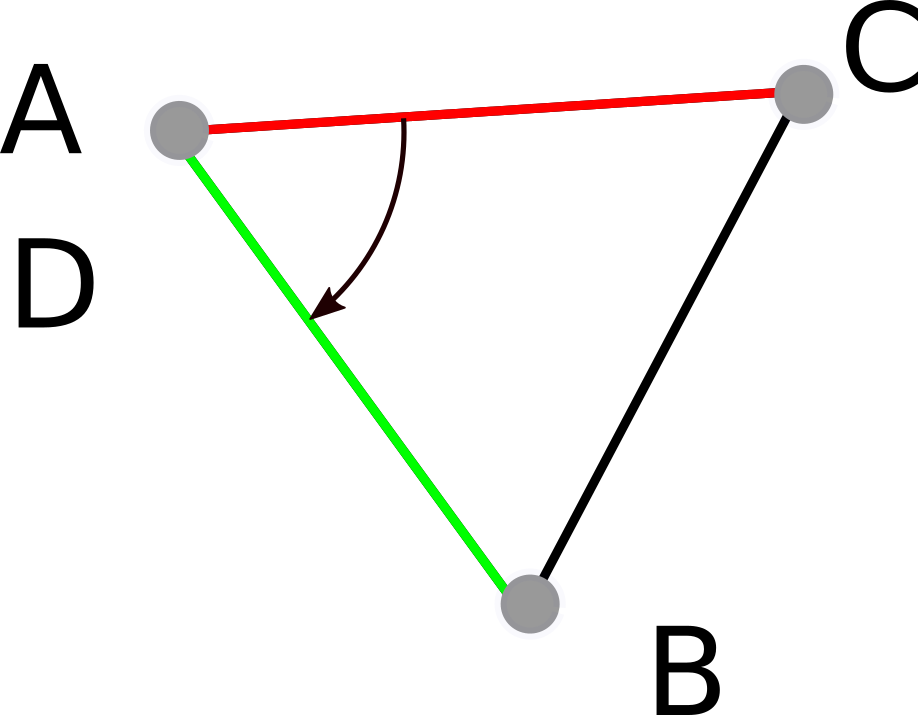
\includegraphics[scale=2]{il}
\caption{\label{intersection_line} the intersection of two lines that are not parallel is a point !}
\end{figure}
\end{itemize}



\subsection{Geometrical Properties}
\label{definition_triangulation}
Then, we define a triangulation Tr on a data set D as a finite set of triangles with points of D as vertices which satisfies some properties :
\begin{enumerate}
\item \ttt{covers\_hull}{Tr D} : the whole convex hull of D is covered by the triangles of Tr
\item \ttt{covers\_vertices}{Tr D} : the points of D are exactly the vertices of the triangle of Tr.
\item \ttt{no\_cover\_intersection}{} : there is no point which is (strictly) in two different triangles of the triangulation. This is written by saying that if two triangles of the triangulation have a common point, then the two triangles are actually the same.
  \item\ttt{no\_point\_on\_segment}{} : no point can be a vertex of a triangle, and on the edge of another triangle (remark : the vertex of a triangle is considered to not be on the edge of this triangle). This is written as: if a vertex of a triangle of the triangulation is in another triangle of the triangulation, then it is a vertex of this triangle.
\item \ttt{triangle\_3\_vertices}{Tr} : every triangle of the triangulation has 3 vertices.
\item \ttt{triangle\_nempty}{Tr} : no triangle of {\tt Tr} is empty (no flat triangle).
\item \ttt{oriented\_triangle\_triangulation}{Tr} : all triangle of the triangulation are well-oriented.

  Remark : by hypothesis, we force \ttt{vertices\_to\_triangle}{} to return a well-oriented triangle so this hypothesis is extremely simple to prove in general.
\end{enumerate}
The two first properties are here to express that the finite set of triangles Tr is indeed a triangulation of the whole data set D, and covers its convex hull with triangles.
Then, the two next properties are here to avoid problems with how the triangles are positioned : 
\begin{enumerate}
\item \ttt{no\_cover\_intersection}{} is here to avoid problems like in Figure \ref{nci} where two triangles {\tt ABC} and {\tt DEF} aren't well positioned; there exists a point {\tt P} that is in both {\tt ABC} and {\tt DEF}.
\\
\begin{figure}[h]
\centering
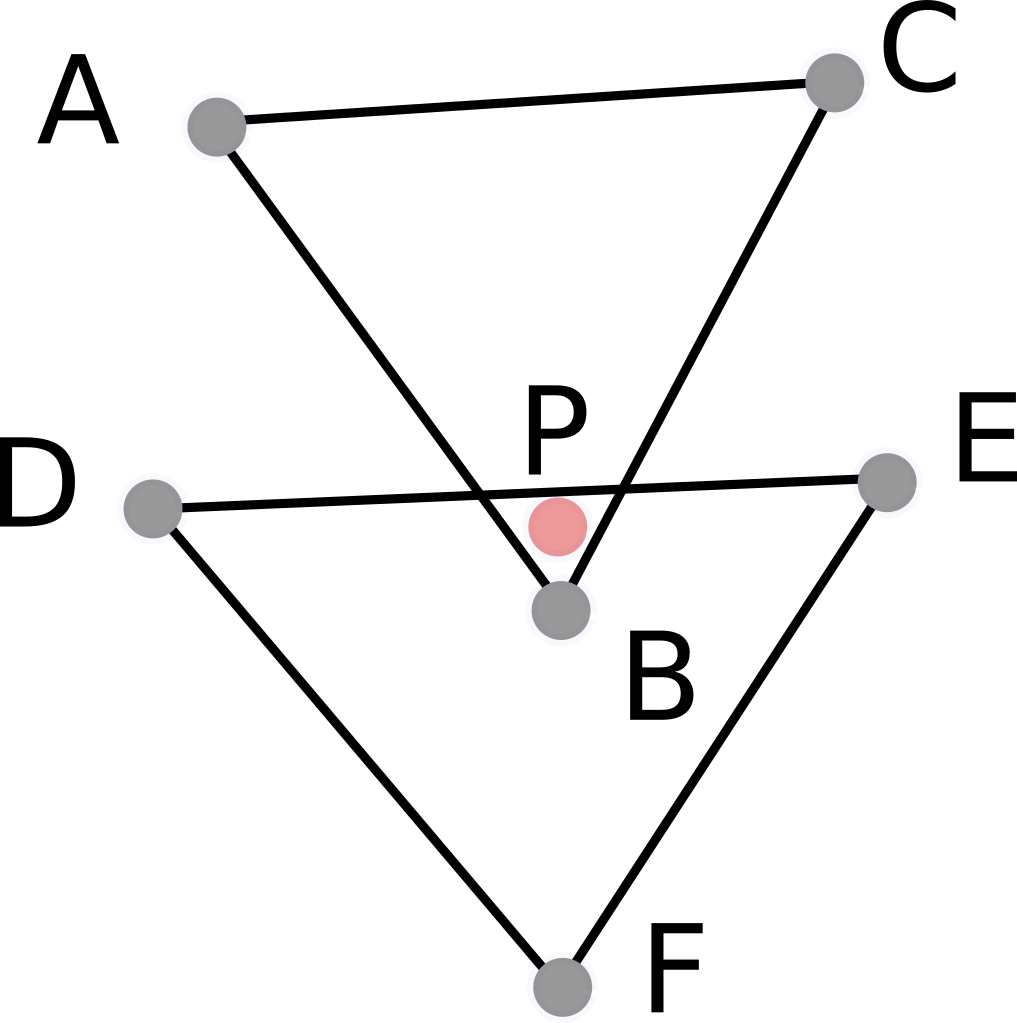
\includegraphics[scale=2]{nci}
\caption{\label{nci} {\tt no\_cover\_intersection}}
\end{figure}
\item \ttt{no\_point\_on\_segment}{} is here to avoid problems like in Figure \ref{nps}, where the vertice {\tt B} of the triangle {\tt ABC} is on the edge {\tt DE} of the triangle {\tt DEF}.
\\
\begin{figure}[h]
\centering
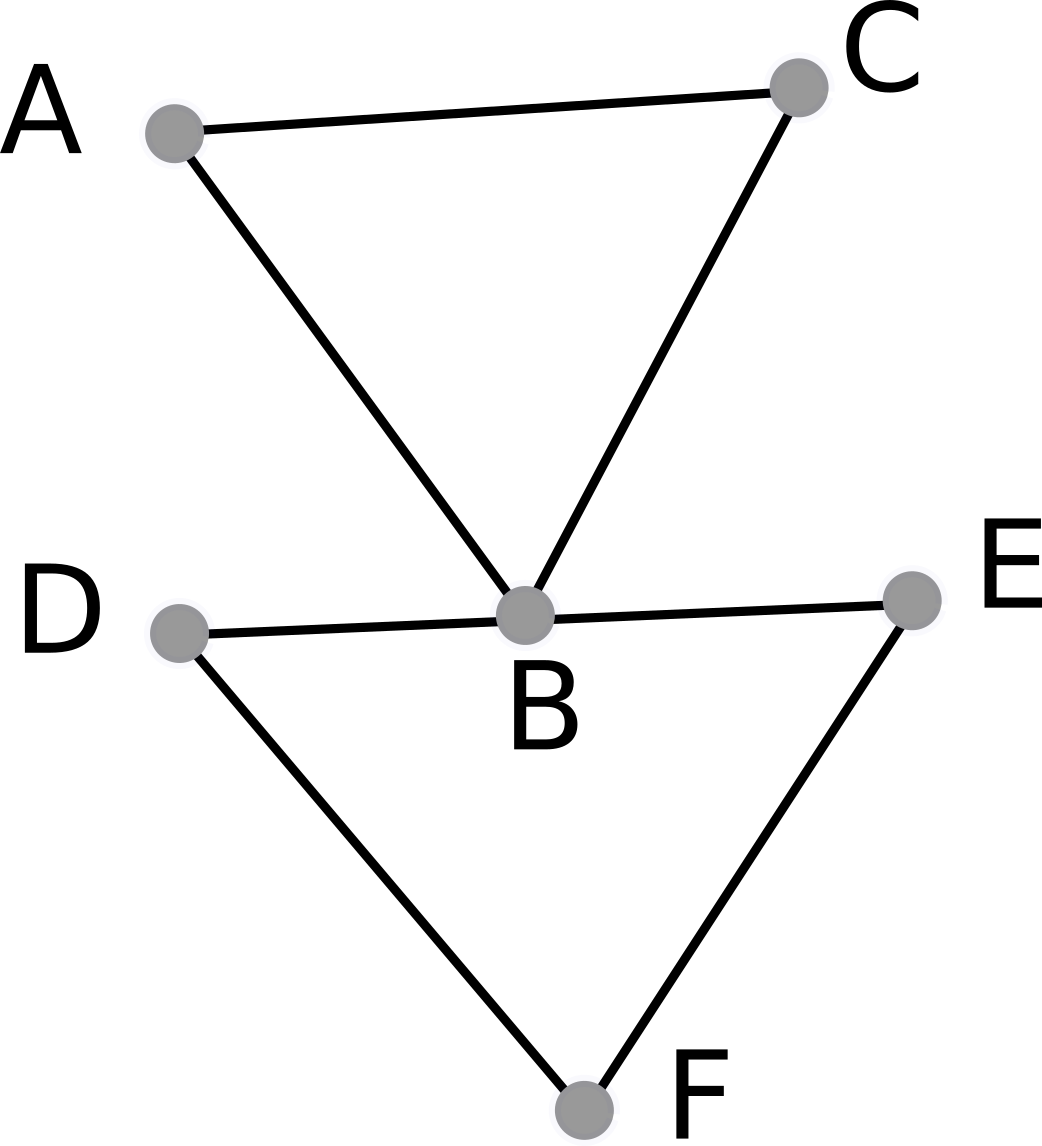
\includegraphics[scale=2]{nps}
\caption{\label{nps} {\tt no\_point\_on\_segment}}
\end{figure}
\end{enumerate}
In both case, the properties are here to assure the fact that the first part of the definition of a triangulation is respected : the intersection of two simplices should either be empty or a face of those simplices.

Finally, the two last properties are here to avoid degenerate cases with the triangles of the triangulation (triangulation shouldn't contain degenerate triangles). It is to be noted that the second property implies the first.

\subsection{Convex Hulls}

The definition of what is a triangulation in dimension 2 requires first to define what is a convex hull of a point set D.
Two different approachs exist :
\begin{enumerate}
\item The first possibility, used by Knuth,  is to define the convex hull as a cyclic sequence S : {\tt (S1; S2; ...; Sn; S1)} of elements of D such that every point of D is ``encompassed'' within S, with {\tt P} being ``encompassed'' within S iff {\tt is\_left\_or\_on\_line Si Si+1 P} is true.
  It's a more geometrical definition.
\item The second possibility is via the notion of barycenter : it is the smallest subset {\tt H} of {\tt D} such that every point of {\tt D} is a barycenter of the points of {\tt H}.
\end{enumerate}

It's the second approach that was used here. It has two main benefits :
\begin{enumerate}
\item First, it is independant of the dimension, whereas the first possibility only works in dimension 2.
\item It is independant to the definition of the geometrical predicates, and those can change (for instance between Knuth's case where points are in general positions and where they are not). 
\end{enumerate}
Also, it is very nicely linked with {\tt oriented\_surface} in dimension 2. Carathéodory's theorem for Convex hulls says :
\begin{theorem}
If a point of $\mathbb{R}^d$ lies in the convex hull of {\tt D}, then it is a barycenter of $d+1$ points of {\tt D}.
\end{theorem}
In dimension 2, this means that every point in the convex hull of {\tt D} is a barycenter of three points of {\tt D} (ie, in a triangle with vertices some points of {\tt D}).
Moreover, there is a nice thing about the coefficients : if $x$ is in $ABC$ then we have :
$$x = x_AA + x_BB + x_CC$$
with : $x_A =\frac{ \text{\tt oriented\_surface B C x}}{\text{\tt oriented\_surface A B C}}$ , (...), which gives a nice relation between the coefficients and the surface of the triangles (Figure \ref{cara}).

\begin{figure}[h]
  \centering

  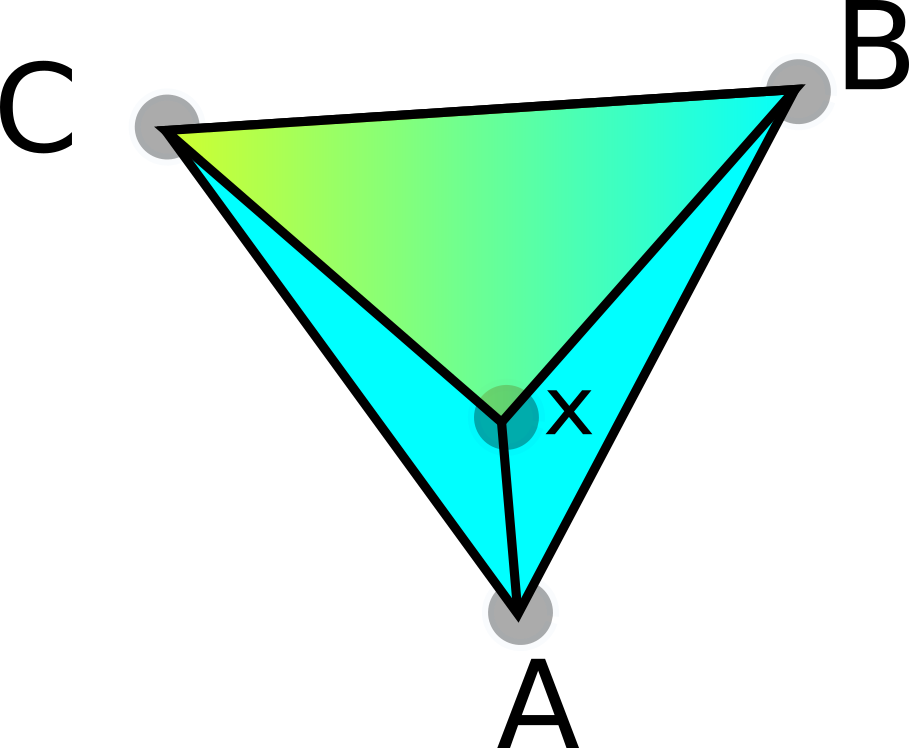
\includegraphics[scale=2]{cara.png}

  \caption{\label{cara} Relation between coefficient and surface}
\end{figure}


\section{Theorems}
\rule{\linewidth}{0.5pt}
\subsection{Adding points}
\label{theorem1}
Following the algorithm described in section \ref{algo} the first step was writing a way to add points to a triangulation : given a triangle $t = ABC$, a point $p$, a triangulation $tr$, {\tt split\_triangle $tr$ $t$ $p$} returns $tr \smallsetminus t \cup \{ABp;pBC;ApC\}$.
\begin{figure}[h]
  \centering
  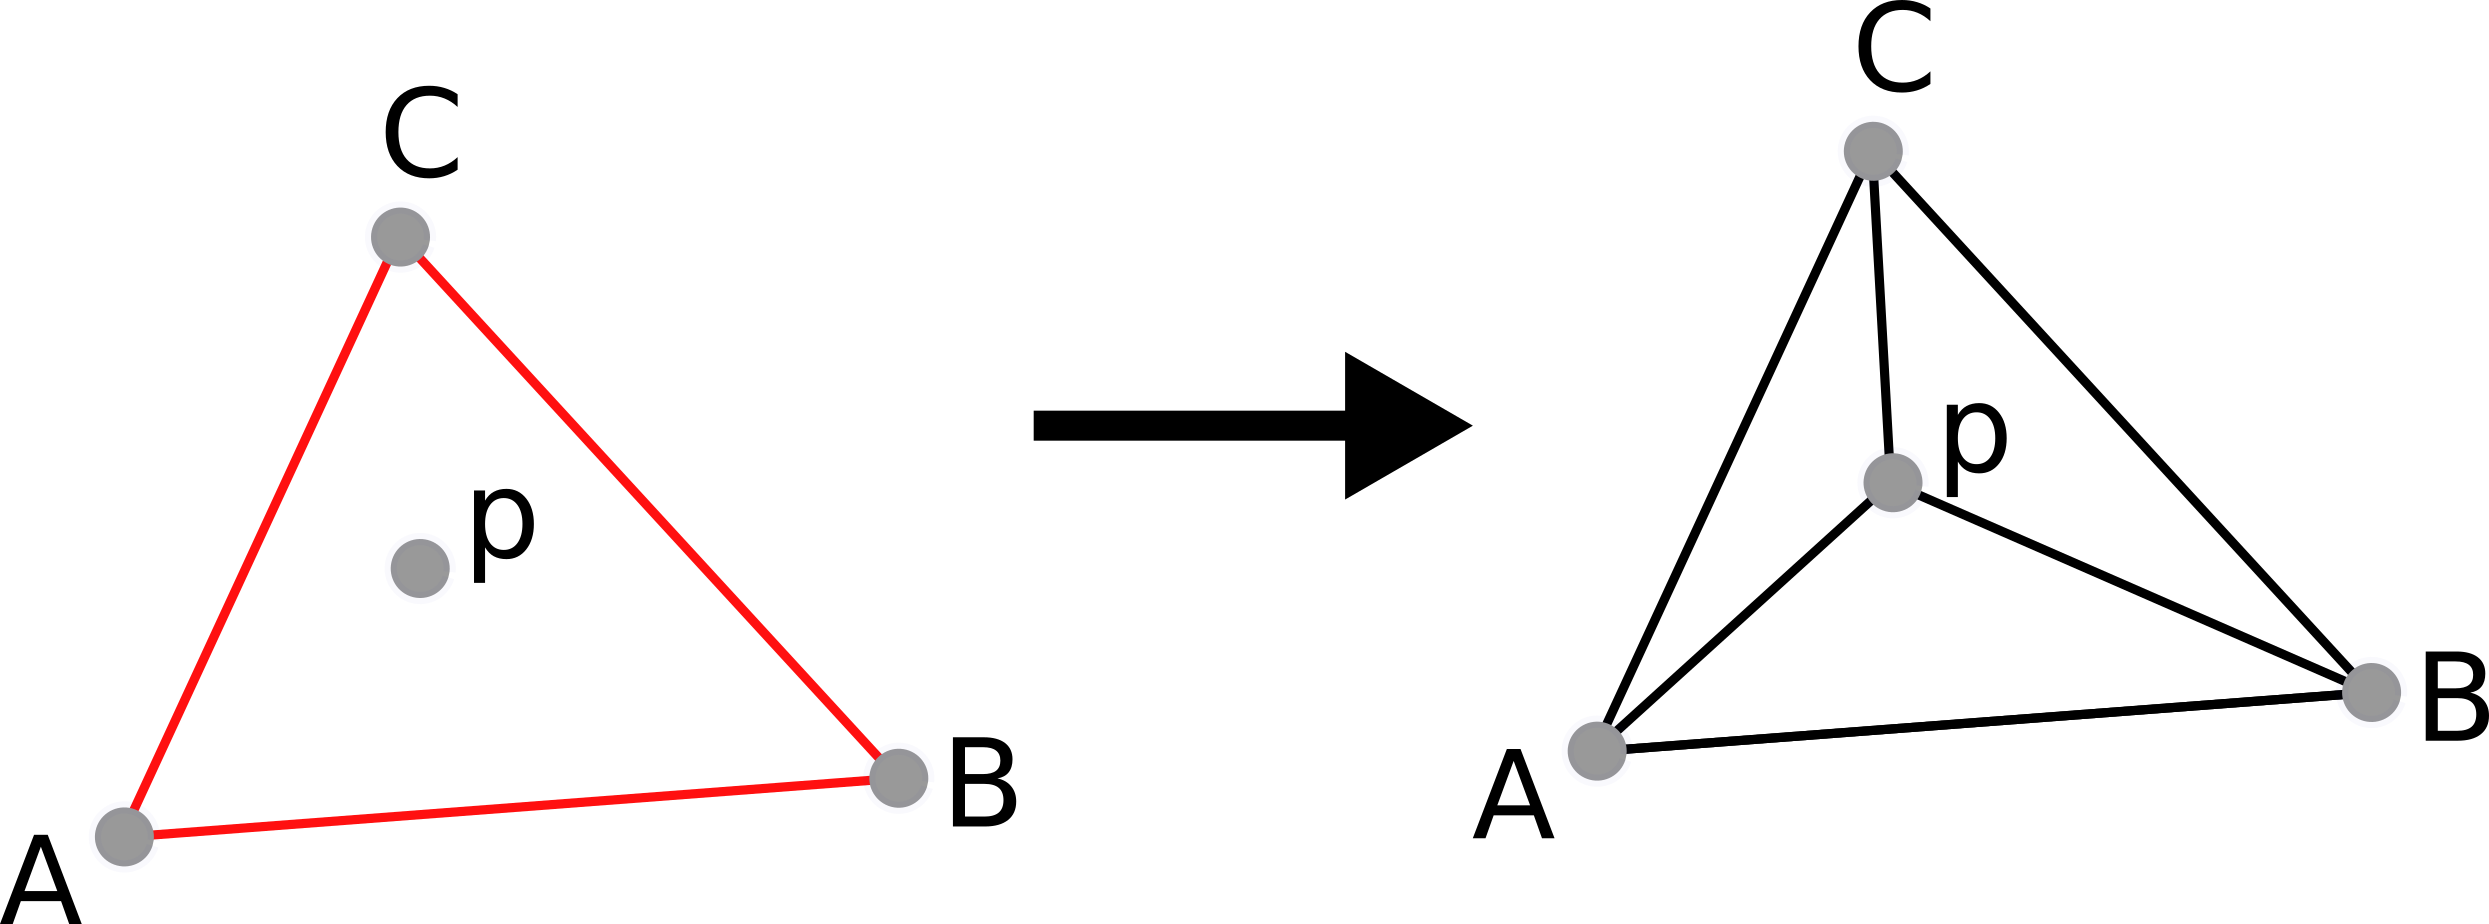
\includegraphics[scale=2]{split_triangle}
    \caption{\label{split_triangle} {\tt split\_triangle}}
\end{figure}

 The theorem proven was :\\
{\tt Theorem triangulation\_split\_triangle:\\
  $\forall$ tr, t, p, d, d != fset0 -> p $\notin$ d $\rightarrow$
                        triangulation tr d $\rightarrow$ t $\in$ tr ->\\
                        in\_triangle t p $\rightarrow$
                        triangulation (split\_triangle tr t p) (p |` d).\\
                       }
In english, this would be written :
\begin{theorem}
  Forall triangulation $tr$ of a nonempty data set $d$,
  triangle of this triangulation t, point strictly in this triangle $p$ ,
  if $p$ is not in $d$, then
  {\tt split\_triangle tr t p} is a triangulation for the data set $d \cup \{p\}$.
\end{theorem}

This is proven by proving the preservation of the six properties described in the definition of a triangulation (Section \ref{definition_triangulation}) :
\subsubsection{For {\tt covers\_hull}}
\label{cvh1}
 For the proof for {\tt covers\_hull}, we prove that $q$ is in the convex hull of $d$ by using the fact that $q$ is in $t$ which is in the triangulation. Then, it comes down to proving three lemmas.

  The first lemma is that if we add to a data set a point that was already in the convex hull of the data set, then the convex hull of this data set doesn't change. Even if looks quite intuitive, the proof of this lemma was actually quite hard to write in {\tt Coq} because of complicated problems of typings within the BigOps part of {\tt MathComp}. 
  
  The second lemma is that a point in a triangle of the triangulation is in the convex hull of the data set of the triangulation.

  The third lemma is that if a point $q$ was in the triangle deleted from the triangulation, then it's in one of the new three triangles. The proof of this lemma is actually the longest proof (for this theorem).
  It's a big case-based reasoning on where $q$ is in the big triangle compared to the segments $Ap$, $Bp$ and $Cp$.
  
  This proof could have been quite smaller, I think, if I used more the tactic {\tt easygeo} I'll speak about in Section \ref{easygeo}. However, I wrote this tactic later and then didn't have the time to redo my proofs using it.

  \subsubsection{For {\tt covers\_vertices}}
  \label{cvv1}
  
  The proof for {\tt covers\_vertices} looks also quite simple. However, it is actually quite long to do with Coq : for instance, when we say that $q$ is the vertex of a triangle $t$, we write that $q$ is in {\tt edges\_set t} and then we have to do a case-based reasoning (is $q$ the first vertex of $t$ or the second or the third...).

  \subsubsection{For {\tt no\_cover\_intersection}}

  For the proof for {\tt no\_cover\_intersection}, it was needed to prove two lemmas.Then it's a big case-based reasoning using the two lemmas, again.

  The first one is stating that if a triangle is (strictly) in a new triangle, then it was in $t$.
  Its proof is quite simple and mainly uses Knuth's $5^{th}$ axiom, the ``transitivity'' (see Section \ref{Hypothesis}).
  
  The second one is stating that a point is in (large definition) one of the new three triangles if and only if it was in (large definition) the triangle deleted from the triangulation. The proof of this lemma was actually very hard and long. It's a case-based reasoning on the position of the point in the big triangle. A trick was used to do the proof : I was certain that some hypotheses were not consistent (and thus I could do a proof by contradiction in some cases), but I couldn't find how to use Knuth's axioms to prove it. After a discussion with Yves, we used an automated tool made by some previous students that tested the consistency of a list of hypotheses (of the type {\tt is\_left\_of A B C} ...) using Knuth's axioms, and finally found how to finish my proof from analysing the results.

  
  
  The proof of the lemma itself was much simpler than the (already proven) reverse and mainly used Knuth's $5^{th}$ axiom, the ``transitivity'' (see Section \ref{Hypothesis}).
  
  \subsubsection{For {\tt no\_point\_on\_segment}}

  The proof for {\tt no\_point\_on\_segment} also comes from a lemma, which is actually the same as another before (being in one of the three new triangles means being in $t$) , but using the large definition of being in a triangle, instead of the strict one.\\
  The lemma is proven using an hypothesis (provable, but I didn't have the time to do it) : if a point is on the edge of one of the three new triangles, then it's either in $t$ on an edge of $t$.
  
  \subsubsection{For {\tt triangles\_3vertices}}

  The proof for {\tt triangles\_3vertices} can look trivial, but, again (like for {\tt covers\_vertices}), it is not. The ``difficulty'' comes from the number of overlapping case-based reasonning on the vertices of the triangles. For this proof, I tried to do as much ``automation'' I could by treating cases together in order to avoid having very long simple proofs.
  
  \subsubsection{For {\tt triangles\_nempty}}

  The proof for {\tt triangles\_nempty} is extremely simple. We know that the triangles we have have all a nonzero oriented surface by hypothesis (definition of {\tt in\_triangle $t$ $p$}), and we deduce from this that there exist at least a point inside them.

  \subsubsection{For {\tt oriented\_triangle\_triangulation}}
  \label{oriented_simple}
  Finally, the proof for {\tt oriented\_triangle\_triangulation} is extremely simple because of the fact we force, by hypothesis, any implementation of {\tt vertices\_to\_triangle} to return a well-oriented triangle. Because of this, the proof is only a very simple case-based reasonning.

  
\subsection{Flipping edges}
The next big step was writing the edge-flipping step {\tt flip\_edge $tr$ $t1$ $t2$ $a$ $b$ $c$ $d$}.
It returns $tr \smallsetminus t1 \smallsetminus t2 \cup \{abd;bcd\}$. It's meant to be called with $t1 = abc$ and $t2=acd$.

\begin{figure}[h]
  \centering
  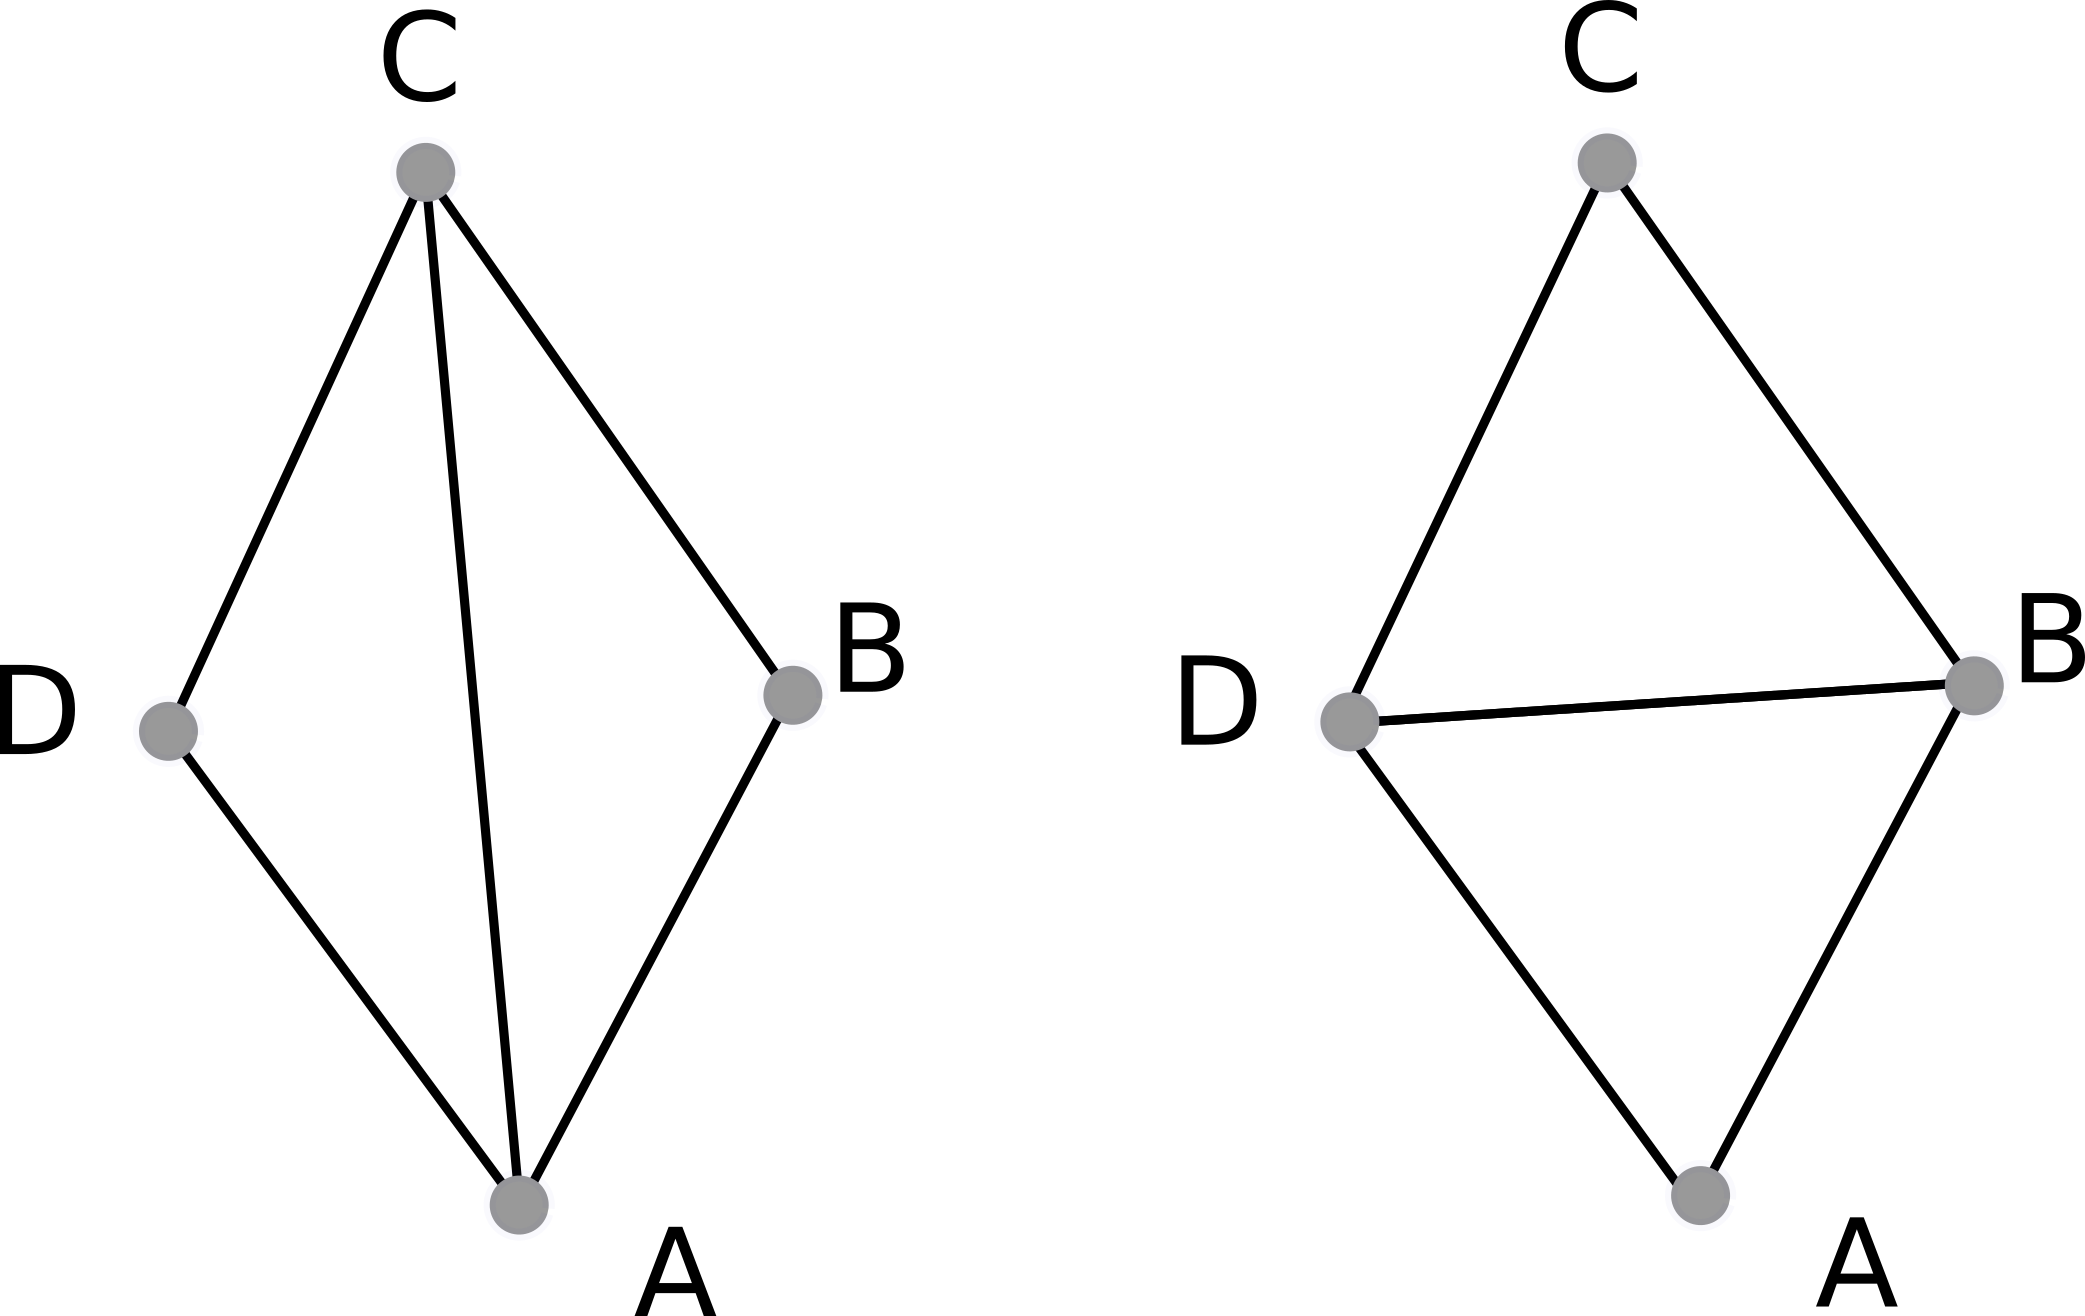
\includegraphics[scale=2]{flip_edge}
    \caption{\label{flip_edge} An edge-flipping step}
\end{figure}

I won't write here the theorem I proved in this report, but, basically, the idea is the same as before (prove that a triangulation in transformed into another triangulation, but with more conditions) :
\begin{itemize}
\item $t_1$ and $t_2$ should be triangles of a triangulation $tr$ on a data set $d$.  
\item $a$,$b$ and $c$ should be points of the data set, vertices of $t_1$ and form a well oriented triangle (we have {\tt is\_left\_of $a$ $b$ $c$})
\item $a$,$c$ and $d$ should be points of the data set, vertices of $t_2$ and form a well oriented triangle (we have {\tt is\_left\_of $a$ $c$ $d$})
\end{itemize}
The way it was written helps with the proofs. It avoid writing things like $t1 = ${\tt vertices\_to\_triangle $a$ $b$ $c$} which would be a problem because of the fact that the order of the vertices of a triangle is important.\\
Again, this is proven by proving the preservation of the six properties.

\subsubsection{For {\tt covers\_hull}} 

For {\tt covers\_hull}, the idea of the proof is quite the same as in Section \ref{cvh1}, but much simpler.
It relies on a lemma : if a point was strictly in one of the previous two triangles, then it is in one of the two new triangles.

The proof of this lemma is also a big case-based reasoning, but it is better automated this time because of the experience I gained between proving all the lemmas necessary for the first theorem.

\subsubsection{For {\tt covers\_vertices}}

The idea of the proof for {\tt covers\_vertices} is the same than in Section \ref{cvv1}. It's a big case-based reasoning that didn't need the proof of another lemma.

\subsubsection{For {\tt no\_cover\_intersection}}

The proof for {\tt no\_cover\_intersection} needed the proof of a two new lemmas.

The first one is : if $q$ was (strictly) in a deleted triangle then it is either in one of the new triangles or on the common edge of those triangles.
\begin{figure}[h]
  \centering
  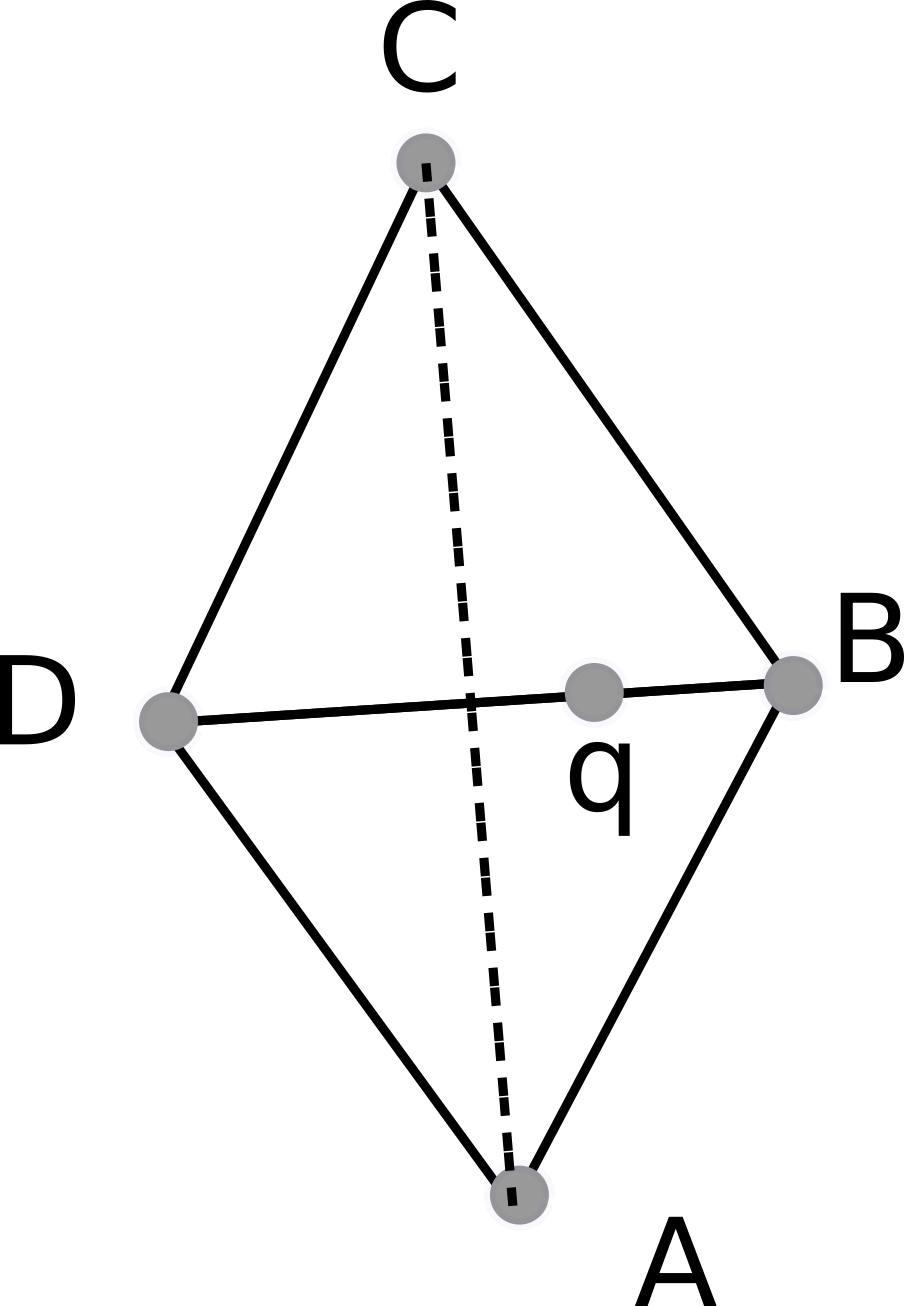
\includegraphics[scale=2]{flip_edge_nci}
    \caption{Here, the point is on the common edge}
\end{figure}

The second lemma proven is : if $a$, $b$ and $c$ are in the vertex set of a triangle $t$, if t is well oriented then forall $p$, p is in {\tt vertices\_to\_triangle $a$ $b$ $c$} if and only if $p$ is in $t$. This looks simple, but actually made me realize a theorem was missing in Cyril Cohen's finmap library , which was quickly added.

The rest of the proof is, as always, just a case-based reasoning.

\subsubsection{For {\tt no\_point\_on\_segment}}
The proof for {\tt no\_point\_on\_segment} is, as usual, a case-based reasoning which needed a new lemma: if a point was in (large definition) a triangle that was deleted from the triangulation, then it's in (large definition) one of the two new triangles.

\subsubsection{For {\tt triangles\_3vertices}, {\tt triangles\_nempty} and {\tt oriented\_triangle\_triangulation}}
The proof for {\tt triangles\_3vertices} is a simple case-based reasoning that I succeed in automating quite a lot, which made it short.

The proof for {\tt triangles\_nempty} was also very short since it was direct from the hypotheses (we know that the oriented surface of the new triangles are positive by hypothesis so, directly, we know that there exist some points in them).

Finally, the proof for {\tt oriented\_triangle\_triangulation} is very direct for the same reason as in Section \ref{oriented_simple}

Proving the conservation of these properties was the main part of the internship. While they looked very simple to prove by hand, proving them in {\tt Coq} was a way more difficult task.

Indeed, {\tt Coq} stops us from using a big part of the mental shortcuts we use to shorten proofs in our head (and it's the good aspect about {\tt Coq}, because it's one of the things that can induce false proofs on paper). One of the most important thing to remember, when proving things with {\tt Coq} and the {\tt Mathematical Component} library, is that it's usually best to try and make a plan for the proof, on paper, and then try to follow this plan.  If something is wrong during the proof and it's not possible to follow the plan, it's that either there is a problem with the proof, or that there is something missing in the library. It's actually very easy to get trapped by {\tt Coq} and try to do the proof by following {\tt Coq} instead of a proof plan!

\section{Instantiation of the model}
\rule{\linewidth}{0.5pt}

The next step of the work was to do an instantiation of the model. For the types :
\begin{itemize}
\item A point is a vector of size 2 of reals : \definition{P}{$'rV[R]_2$. }
\item A triangle is a vector of size 3 of points : \definition{T}{$'rV[P]_3$. }
\item An edge is a vector of size 2 of points : \definition{E}{$'rV[P]_2$. }
\end{itemize}
For the implementation of the functions, with ord$nx$ being the $x+1{th}$ element of the Ordinal $n$ (a well ordered set with $n$ elements )::
 \begin{itemize}
  \item \definition{xCoord (p : P)}{p ord10 ord20} \\( in {\tt MathComp}, a vector of elements of $\mathbb{R}$ of size 2 is a function of the Ordinal 1 in the Ordinal 2 in $\mathbb{R}$). 
  \item \definition{yCoord (p : P)}{p ord10 ord21}.
   \item \definition{vertex (t : T)}{t ord10} which gives a function of the Ordinal 3 in P.
\item {\tt oriented\_surface a b c} can be defined as the determinant of the matrix :
  $$\begin{matrix}
1 & \text{{\tt xCoord  a}} & \text{{\tt yCoord  a}}\\
1 & \text{{\tt xCoord  b}} & \text{{\tt yCoord  b}}\\
1 & \text{{\tt xCoord  c}} & \text{{\tt yCoord  c}}
\end{matrix}$$\\
This makes it so that most proofs on {\tt oriented\_surface} are very nice to do : one only needs to expand the determinant and then use automatic tactics on rings. The only difficulty was to add the ring on which we worked ($\mathbb{R}$ with the usual operations) so that the automatic tactic {\tt ring} worked.

\item The predicate {\tt in\_circle p a b c}, testing if p is in the circumcircle of the triangle {\tt abc} can also be defined as testing if the determinant of this matrix is negative :

  $$\begin{matrix}
1 & \text{{\tt xCoord  p}} & \text{{\tt yCoord  p}}& \text{{\tt (xCoord  p)$^2$ + (yCoord  p)$^2$}}\\
1 & \text{{\tt xCoord  a}} & \text{{\tt yCoord  a}}& \text{{\tt (xCoord  a)$^2$ + (yCoord  a)$^2$}}\\
1 & \text{{\tt xCoord  b}} & \text{{\tt yCoord  b}}& \text{{\tt (xCoord  b)$^2$ + (yCoord  b)$^2$}}\\
1 & \text{{\tt xCoord  c}} & \text{{\tt yCoord  c}}& \text{{\tt (xCoord  c)$^2$ + (yCoord  c)$^2$}}
\end{matrix}$$\\
\item The implementations of {\tt vertices\_to\_triangle} and {\tt vertices\_to\_edge} were not trivial to do.

  First, for {\tt vertices\_to\_triangle a b c}, since we require in the formalisation that any triangle obtained by {\tt vertices\_to\_triangle} should be well-oriented, we have to check if $abc$ form a well-oriented triangle. If yes, we return $abc$, else we return $bac$ which will be oriented by definition of the {\tt is\_left\_of} predicate.

  Then, for {\tt vertices\_to\_edge}, we require, for every {\tt a} and {\tt b}, that {\tt vertices\_to\_edge a b } = {\tt vertices\_to\_edge b a}. To do that, we define a lexicographic order on the points. Then, if {\tt a} $\leq$ {\tt b} we return {\tt ab}, else we return {\tt ba}.
\end{itemize}
The proofs can be grouped in several types :
\begin{enumerate}
\item The proofs on the geometrical predicates (for instance, the fact that {\tt oriented\_surface a b c} = {\tt oriented\_surface b c a} = {- \tt oriented\_surface b a c}) were quite easy because of the fact that proofs on determinants only require to expand the determinants and then do some calculus, which is automatic with the tactic {\tt ring}. I reused some work done by a previous intern, Wassim Haffaf, in this part (the way he expanded 3 x 3 determinants for instance).
\item The proofs requiring more geometrical facts (a good example of this is the proof of the hypothesis {\tt on\_edge\_on\_line}, see Section \ref{Hypothesis}).

  Those were way harder and I didn't have the time to finish them all. {\tt on\_edge\_on\_line} and {\tt on\_line\_on\_edge} are two examples of proofs I tried to do but couldn't finish because I was running out of time and the proofs were very difficult.
  \item The proofs on the functions (for instance, the proofs on {\tt edge\_set} and {\tt vertices\_to\_triangle}). Those were generally simpler than the previous type of proofs (the difficulty coming more from the use of {\tt Coq} and how to do case-based reasoning in an intelligent/automatic way, more than from geometrical problems). I still couldn't finish them all , but I managed to do a good part of them. 

  \item The proofs of Knuth's axioms.

    I didn't have time to begin proving these at all. However, some (most ?) of them could probably be recovered from previous work done by other students (for instance, the work on convex hulls done by David Pichardie (see \cite{Hull}).
  \end{enumerate}

  The instanciation of the model was a very interesting part of the internship. When I tried to do it, I realised a lot of problems about the first version of my formalisation of the Delaunay triangulation : some hypothesis were not precise enough, some were even false (for instance, a problem I had was that it's sometimes hard to realise that triangles can be flat when thinking about hypotheses), and I had to rethink a lot of hypotheses and proofs.


%\section{Examples of proofs}
%\rule{\linewidth}{0.5pt}
%\label{example}
%\label{easygeo}*)
\newpage
\section{Conclusion}
\rule{\linewidth}{0.5pt}
\subsection{Possible improvements}

There are some clear possible paths of improvement for my work. First, all the proofs aren't finished. Then, the next step for me would have been to implement, in {\tt Coq}, from the different steps. The biggest difficulty would have been to prove the termination of the algorithm which transform a random triangulation into a Delaunay triangulation: the way it is done is by saying that, during the algorithm, the lifted image of the triangulation on the unit paraboloid is a quantity that is decreasing. A more detailed explanation of this fact can be found here :
\href{https://www.ti.inf.ethz.ch/ew/Lehre/CG13/lecture/Chapter 6.pdf}{https://www.ti.inf.ethz.ch/ew/Lehre/CG13/lecture/Chapter 6.pdf}.

Then, when this is finished, there are some other possibilities to extend my work :
\begin{enumerate}
\item First, a good way to extend this work could be to generalize the formalisation of Delaunay Triangulations to algorithm that work in higher dimension. In fact, the method I formalised, the incremental construction using flips, can be generalized in dimension 3 or highed (\cite{CompGeoAlgo}). However, the complexity can be exponential in the dimension (as shown in \cite{IncrementalDimension})
\item Another idea could be to try and formalise other Delaunay Triangulation algorithm. It is shown in \cite{Comparison} that the better method to compute Delaunay Triangulation is a Divide and Conquer algorithm presented in \cite{AlgoDivide}. An implementation of this algorithm is presented here :\\
  \href{http://www.geom.uiuc.edu/~samuelp/del_project.html}{{\tt http://www.geom.uiuc.edu/$\sim$samuelp/del\_project.html}}
\end{enumerate}


\subsection{Perspectives}

There are also some things that could be changed about the work I've done.

First, my proficiency with {\tt Coq} and, especially, {\tt SSReflect} changed during the internship. I already followed, before it, a one week course on {\tt SSReflect} and I've done an internship in IRISA,Rennes where I've used {\tt Coq} to do proofs on programs. However, this was not comparable to how I had to use {\tt Coq} during this internship. As such, at the beginning of the internship, I've taken lots of time to prove things that would have been very easy for me at the end of the internship.

  Moreover, the proofs I've done at the end of the internship are ``cleaner'' than the one I've done at the beginning at the internship, taking advantage from the use of the syntax of {\tt SSReflect} and of tricks like the use of the tactic {\tt try}.

  Also, near the end of the internship, I wrote a little (very simple) tactic, which I named {\tt easygeo} \label{easygeo}. I realised, maybe a little too late, that I spent too much time thinking on how to use my hypotheses. Indeed, there were lots of cases where I wanted to use a theorem, with a pack of hypotheses. But, instead of having, for instance, {\tt is\_left\_of b c a}, I had, as an hypothesis, {\tt is\_left\_of a b c} (which we know is equivalent). Thus, before applying the theorem I wanted to apply, I had to spend time rewriting my hypothesis with lemmas. The goal of this tactis, {\tt easygeo}, was to basically use brute force to solve some cases: for instance, if I wanted to prove {\tt is\_left\_of a b c} and I had, {\tt is\_left\_of b c a}, the tactic would solve instantly the goal. Since I wrote this tactic very late in the internship, this tactic isn't (much) used in most of the proofs.

\section{Acknowledgements}
I would like to thank a lot my supervisor, Yves Bertot for all the time he spent helping me during this internship, and all the good references he gave to help me. I would also like to acknowledge Cyril Cohen, who helped me a lot during the internship and Laurence Rideau, who helped me find this internship. I also want to thank all the other members of the MARELLE team at INRIA Sophia-Antipolis for their friendly welcome and help.

I would also like to acknowledge Pierre Alliez, from the TITANE team at INRIA Sophia-Antipolis for the nice and helpful discussion he granted us which conforted us in the direction we were taking in this research.

\newpage
\bibliographystyle{alpha}
\bibliography{Report}
\end{document}



